%%%%%%%%%%%%%%%%%%%%%%%%%%%%%%%%%%%%%%%%%%%%%%%%%%%%%%%%%%%%%%%%%%%%%%%%
% Plantilla TFG/TFM
% Escuela Politécnica Superior de la Universidad de Alicante
% Realizado por: Jose Manuel Requena Plens
% Contacto: info@jmrplens.com / Telegram:@jmrplens
%%%%%%%%%%%%%%%%%%%%%%%%%%%%%%%%%%%%%%%%%%%%%%%%%%%%%%%%%%%%%%%%%%%%%%%%

\chapter{Anexo}
\section{Vicisitudes durante el desarrollo}
El primer problema que me gustaría comentar en el anexo fue la sobrestimación de mis capacidades. Por lo que me ha comentado mi tutor, es algo que suele pasar, sobretodo cuando eres una persona sin experiencia en el sector. Desde el principio del proyecto apunté a hacer cosas que eran extremadamente difíciles, pero por suerte mi tutor supo cómo orientarme en el camino y pararme los pies en ciertos momentos, ya que de no haber sido así, es probable que no hubiese acabado el proyecto. 
\\
Otra parte en la que sobreestimé mis capacidades fue a la hora de desarrollar el motor de videojuegos. Ciertamente comencé a ver las clases de \cite{CursoMotorC++} en verano, pero cuando comenzó el curso fue cuando comencé a desarrollarlo. Pensaba que en un mes de trabajo habría terminado, sin embargo, no fue hasta mediados de noviembre que terminé por completo el desarrollo del mismo. Por supuesto, sin contar las posteriores correcciones.
\\
Además, también sobreestimé mis conocimientos sobre estadística, probabilidad y programación. Es cierto que es algo que siempre me han gustado, y a raíz de eso y tener tanto relación con la \gls{ia}, fue por lo que elegí el tema del \gls{tfg}, pero entender y desarrollar el algoritmo de \textit{backpropagation} fue algo que me llevó mucho más tiempo del que habría imaginado.

Otro de los problemas fue la pérdida del proyecto. Como ya he mencionado en el apartado de herramientas de trabajo, yo he desarrollado este proyecto con Linux, pero por motivos relacionados con la carrera, es necesario que también tenga instalado Windows en el ordenador. Después de una actualización, este último dejó de funcionar, y cuando opté por solucionar el error, se cargó la partición de Linux. Por suerte, todo el trabajo del \gls{tfg} estaba bajo el control de Git, y en la nube de GitHub, por lo que los daños en ese sentido eran mínimos. Pero tuve que invertir una cantidad de tiempo considerable en recuperar el resto de cosas de mi ordenador que no tenían una copia de seguridad alguna. Desde luego que ahora tengo más cuidado con hacer copias de seguridad de las cosas importantes.
\\
No voy a contar cómo fue la recuperación del sistema operativo ya que no procede en esta memoria, pero esto juntado con los trabajos de las asignaturas de la universidad, me hizo perder más de una semana.

Por último quiero comentar que este largo desarrollo ha sido posible porque este es mi quinto año de carrera, sólo tenía dos asignaturas que cursar en todo el año, y por eso me he permitido la licencia de dedicarle tanto tiempo al proyecto. Por otro lado, si ya hubiese tenido conocimientos previos más avanzados sobre \gls{ia}, y sobre motores de videojuegos, el desarrollo podría haberse acortado meses, sin embargo, es algo que he hecho con ganas y me ha servido para tener una experiencia que tendrá mucha utilidad en mi futuro.

\section{Cómo probar el juego}
Puede darse el caso de que quieras probar el juego, por lo que te daré las instrucciones para compilarlo, y además, los controles del juego.
Compilar es tan sencillo como entrar en la carpeta donde se ubique el Makefile y ejecutar desde una terminal \texttt{make libs \&\& make}, se generará un ejecutable llamado game y tendrás que ejecutar desde ese mismo directorio \texttt{./game}. Sin embargo, puede que tengas algún problema en la compilación, siempre y cuando no tengas instalado X11, GLFW, OpenGL y GLEW. Para instalar estas librerías en Linux, dependerá de tu distribución, pero lo que tienes que hacer es buscar con tu gestor de paquetes cómo se llaman en tu distribución estas librerías y descargarlas.

Para jugar al juego, una vez compilado, lo que harás será seleccionar la opción ``Play'', esta sirve para jugar una \gls{ia} contra otra. Mientras que la opción ``Arena'', sirve para recoger datos en un archivo dataset, con el cual podrás entrar en la siguiente opción llamada ``Train''. Esta última te llevará a un nuevo menú en el que podrás ajustar diferentes parámetros para el entrenamiento mediante \textit{backpropagation}. Todo esto se ve en la figura \ref{Menu inicial definitivo}.
\begin{figure}[H]
	\centering
	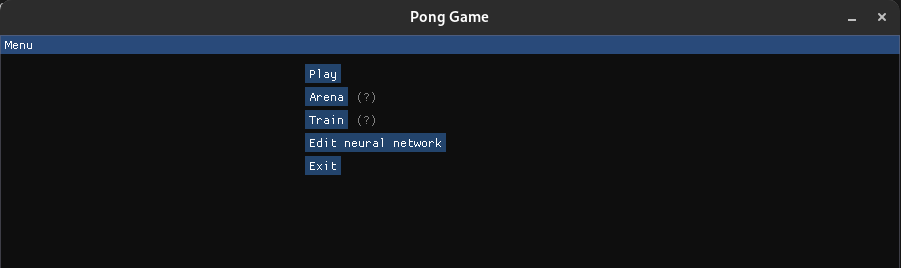
\includegraphics[width=15cm]{archivos/imagenes/menu-inicia-definitivo.png}
	\caption{Menú inicial definitivo.}
	\label{Menu inicial definitivo}
\end{figure}

En el menú de entrenamiento aparecen los ajustes recomendados, pero puedes variarlos para probar cómo cambia el error de la red en tiempo real, tanto el \textit{learning rate} como la cantidad de muestras de cada tipo que se le entregan al agente durante el entrenamiento.

Por último, las teclas para manejar al jugador de la izquierda son \textbf{w} y \textbf{s}, y para el jugador de la derecha son \textbf{o} y \textbf{l}.